% AA-55
\chapter{Grafy McKaya i afiniczne diagramy Dynkina}
\label{aa:ch:mckay}

W rozdziałach~\ref{aa:ch:binary-polyhedral}--\ref{aa:ch:exceptional-invariants}
sklasyfikowaliśmy skończone podgrupy $\operatorname{SL}_2(\mathbb C)$
i wyznaczyliśmy ich pierścienie niezmienników. Teraz
odczytamy tę samą listę typów z teorii reprezentacji.
Nie będziemy zakładać klasyfikacji diagramów Dynkina.

\section{Macierz McKaya}

\begin{definicja}[Graf McKaya]
\label{aa:def:mckay}
Niech $G\le\operatorname{SL}_2(\mathbb C)$ będzie skończona,
$V=\mathbb C^2$ jej naturalną reprezentacją, a
$V_0,\ldots,V_s$ pełną listą parami nierównoważnych
zespolonych reprezentacji nieprzywiedlnych, przy czym
$V_0=\mathbb C$ jest reprezentacją trywialną.
Macierzą McKaya nazywamy macierz $A=(a_{ij})$ określoną przez
\[
 V\otimes V_i\simeq\bigoplus_{j=0}^s V_j^{\oplus a_{ij}}.
\]
Graf McKaya ma wierzchołki $0,\ldots,s$, a liczba
skierowanych krawędzi od $i$ do $j$ wynosi $a_{ij}$.
Gdy $A$ jest symetryczna, dla $i\ne j$ będziemy
rysować $a_{ij}$ krawędzi nieskierowanych; wpis
$a_{ii}$ zachowamy jako krotność pętli.
\end{definicja}

\begin{twierdzenie}[Własności macierzy McKaya]
\label{aa:tw:mckay-properties}
Niech $G,V,V_i,A$ będą jak w
Definicji~\ref{aa:def:mckay}, a $d_i=\dim V_i$.
Wówczas $A$ jest symetryczna, graf jest spójny,
$Ad=2d$ dla $d=(d_i)_{i=0}^s$ oraz
$\sum_i d_i^2=|G|$. Jeżeli $-I\in G$, graf jest dwudzielny
i nie ma pętli.
\end{twierdzenie}
\begin{proof}
Po sprzężeniu możemy przyjąć $G\le\operatorname{SU}(2)$
na mocy Twierdzenia~\ref{aa:tw:binary-unitary}.
Wartości własne $g\in G$ mają postać $\lambda,\lambda^{-1}$
dla $|\lambda|=1$. Zatem charakter $\chi_V(g)$ jest rzeczywisty,
a wartość $2$ przyjmuje tylko dla $g=I$: wówczas
$\operatorname{Re}\lambda=1$ wymusza $\lambda=1$,
a unitarna macierz o obu wartościach własnych równych $1$
jest identycznością.
Z formuły na krotności
(Twierdzenie~\ref{aa:tw:multiplicities}) mamy
\[
 a_{ij}=\frac1{|G|}\sum_{g\in G}
   \chi_V(g)\chi_i(g)\overline{\chi_j(g)}.
\]
Ponieważ $\chi_V$ jest rzeczywisty, $a_{ji}=\overline{a_{ij}}=a_{ij}$.
Porównanie wymiarów w definicji daje $2d_i=\sum_j a_{ij}d_j$.
Rozkład reprezentacji regularnej z
Twierdzenia~\ref{aa:tw:regular-character} daje
$|G|=\sum_i d_i^2$.

Dla spójności załóżmy, że $j$ nie należy do składowej
wierzchołka $0$. Indukcja według $k$ pokazuje, że
każdy składnik nieprzywiedlny $V^{\otimes k}$
jest w tej składowej: dla $k=0$ jest to reprezentacja
trywialna, a iloczyn tensorowy z $V$ przechodzi
wyłącznie do sąsiadów. W konsekwencji dla każdego $k\ge0$
\[
 0=\frac1{|G|}\sum_{g\in G}\chi_V(g)^k\overline{\chi_j(g)}.
\]
Niech $T=\{\chi_V(g):g\in G\}$ i
$p(t)=\prod_{u\in T\setminus\{2\}}(t-u)/(2-u)$.
Wielomian ten przyjmuje wartość $1$ w $2$ i $0$ w pozostałych
punktach $T$. Biorąc kombinację powyższych równości
ze współczynnikami $p$, otrzymujemy
$0=\overline{\chi_j(I)}/|G|=d_j/|G|$, sprzeczność.

Gdy $-I\in G$, jego działanie na $V_i$ jest skalarem
$\varepsilon_i\in\{1,-1\}$ na mocy lematu Schura
i równości $(-I)^2=I$. Na $V\otimes V_i$ działa jako
$-\varepsilon_i$. Jeżeli $a_{ij}>0$, to
$\varepsilon_j=-\varepsilon_i$. Podział wierzchołków
według znaku jest więc podziałem dwudzielnym.
\end{proof}

\begin{lemat}[Podgraf o dodatnim wektorze wymiarów]
\label{aa:lem:mckay-subgraph}
Niech $A$ będzie symetryczną macierzą stopnia $N\ge1$
o nieujemnych współczynnikach całkowitych, której
graf jest spójny.
Załóżmy $Ad=2d$ dla wektora $d>0$ (wszystkie współrzędne
dodatnie). Niech $B$ będzie symetryczną macierzą
podgrafu na niepustym podzbiorze $S$ wierzchołków,
czyli $0\le B_{ij}\le A_{ij}$ dla $i,j\in S$.
Jeśli $Bu=2u$ dla $u>0$, to $S$ jest całym zbiorem
wierzchołków i $B=A$.
\end{lemat}
\begin{proof}
Dla ograniczenia $d_S$ mamy dla każdego $i\in S$
\[
 (2d_S-Bd_S)_i=
 \sum_{j\in S}(A_{ij}-B_{ij})d_j+
 \sum_{j\notin S}A_{ij}d_j\ge0.
\]
Nierówność wynika z założeń o współczynnikach i o $d$. Ponadto
$u^{\mathsf T}(2d_S-Bd_S)=(2u-Bu)^{\mathsf T}d_S=0$.
Każda współrzędna różnicy jest nieujemna, a każda
współrzędna $u$ dodatnia, więc $Bd_S=2d_S$.
Ponieważ wszystkie $d_i>0$, żadna pominięta krawędź
ani zmniejszenie krotności nie jest możliwe.
Zatem z $S$ nie wychodzi żadna krawędź, a spójność daje
$S$ równy całemu zbiorowi.
\end{proof}

\section{Klasyfikacja grafów bez pętli}

\begin{twierdzenie}[Klasyfikacja kombinatoryczna]
\label{aa:tw:mckay-graphs}
Niech $A$ będzie symetryczną macierzą stopnia $N\ge1$
o nieujemnych współczynnikach całkowitych, z zerami na przekątnej,
o spójnym grafie i niech $Ad=2d$ dla $d>0$.
Wówczas graf jest jednym z następujących:
\begin{enumerate}
\item dwa wierzchołki połączone dwiema krawędziami
      ($\widetilde A_1$) lub cykl o $m\ge3$ wierzchołkach
      ($\widetilde A_{m-1}$);
\item gwiazda z czterema liśćmi ($\widetilde D_4$)
      lub ścieżka z $k\ge1$ krawędziami, do której
      każdego końca dołączono po dwa liście
      ($\widetilde D_{k+4}$);
\item drzewo o jednym wierzchołku stopnia trzy,
      z ramionami długości odpowiednio $(2,2,2)$,
      $(1,3,3)$ albo $(1,2,5)$
      ($\widetilde E_6,\widetilde E_7,\widetilde E_8$).
\end{enumerate}
Długość ramienia oznacza liczbę krawędzi od wierzchołka
stopnia trzy do liścia. Każdy wymieniony graf ma
dodatni wektor $d$ spełniający $Ad=2d$, jednoznaczny
z dokładnością do dodatniego mnożnika.
\end{twierdzenie}
\begin{proof}
Jeśli istnieje krawędź krotności co najmniej dwa,
podgraf dwóch wierzchołków z dwiema krawędziami
ma dodatni wektor $(1,1)$. Lemat~\ref{aa:lem:mckay-subgraph}
wymusza równość z tym podgrafem.
Odtąd graf jest prosty. Nie może mieć jednego
wierzchołka: wtedy $A=(0)$ i $Ad=0\ne2d$.
Jeśli zawiera cykl, wybieramy
jego krawędzie i wierzchołki. Wektor samych jedynek
spełnia na cyklu wymagane równanie, więc ten sam
lemat daje równość grafu z cyklem.

Pozostał przypadek drzewa. Jeśli jakiś wierzchołek ma
stopień co najmniej cztery, wybieramy go i czterech
sąsiadów z krawędziami do niego. Wektor o wartości
$2$ w centrum i $1$ w liściach spełnia równanie.
Lemat wyklucza wszystkie dodatkowe krawędzie i wierzchołki.
Jeżeli są przynajmniej dwa wierzchołki stopnia trzy,
wybieramy parę o najmniejszej odległości. Wewnętrzne
wierzchołki ich jedynej ścieżki mają stopień dwa,
gdyż w przeciwnym razie istniałaby bliższa para.
Do każdego końca ścieżki dołączamy jego dwóch sąsiadów
spoza ścieżki; są oni parami różni, ponieważ graf
nie ma cykli. Na tym podgrafie nadajemy wartości
$2$ wszystkim wierzchołkom ścieżki oraz $1$ czterem
nowym liściom. Wewnętrzny wierzchołek ścieżki ma
sumę sąsiadów $2+2=4$, jej koniec $2+1+1=4$,
a liść ma sąsiada o wartości $2$.
Z lematu wynika równość z całym grafem.

Drzewo bez rozgałęzienia byłoby ścieżką.
Po oznaczeniu jej wartości przez $d_1,\ldots,d_l$
i dodaniu $d_0=d_{l+1}=0$, równania
$2d_j=d_{j-1}+d_{j+1}$ wymuszają stałe różnice
$d_j-d_{j-1}$. Z obu zer na końcach wynika, że różnica
jest zero, co przeczy dodatniości.
Pozostaje dokładnie jeden wierzchołek stopnia trzy.
Po jego usunięciu otrzymujemy trzy składowe: sąsiedzi
nie mogą należeć do tej samej składowej, bo powstałby
cykl. Każda składowa jest ścieżką (być może
jednowierzchołkową), a dawny sąsiad wierzchołka
centralnego jest jej końcem, bo utracił jedną krawędź.
Niech wierzchołek centralny ma wartość $h>0$,
a ramiona mają długości $l_1,l_2,l_3\ge1$. Na ramieniu długości $l$ oznaczamy
wartości przez $b_0=h,b_1,\ldots,b_l,b_{l+1}=0$.
Równanie $2b_j=b_{j-1}+b_{j+1}$ wymusza
$b_j=h(l+1-j)/(l+1)$. W centrum otrzymujemy
\[
 2h=\sum_{i=1}^3 h\frac{l_i}{l_i+1},
 \qquad
 \sum_{i=1}^3\frac1{l_i+1}=1.
\]
Uporządkujmy $a=l_1+1\le b=l_2+1\le c=l_3+1$.
Gdy $a\ge4$, suma nie przekracza $3/4$.
Dla $a=3$ wszystkie trzy składniki nie przekraczają
$1/3$, więc $a=b=c=3$. Dla $a=2$ mamy
$1/b+1/c=1/2$. Wartość $b=2$ jest niemożliwa,
a $b\ge5$ daje sumę co najwyżej $2/5$.
Jeśli $b=3$, to $c=6$; jeśli $b=4$, to $c=4$.
Otrzymujemy dokładnie podane trzy zestawy ramion.
Wzór na $b_j$ i równanie centralne dowodzą też istnienia
dodatniego wektora dla każdego z nich. Dla pozostałych
grafów istnienie pokazują skonstruowane wcześniej
wektory: same jedynki dla typu $A$, dwójki na ścieżce
i jedynki w liściach dla typu $D$ (w gwieździe
dwójka tylko w centrum).

Na koniec, jeśli $u,v>0$ spełniają $Au=2u$, $Av=2v$,
to dla $t=\min_i u_i/v_i$ wektor $w=u-tv$ jest
nieujemny, ma współrzędną zerową i spełnia $Aw=2w$.
Jeśli $w_i=0$, to $\sum_j a_{ij}w_j=0$, więc
$w_j=0$ dla wszystkich sąsiadów $i$. Spójność
przenosi zero na wszystkie wierzchołki, zatem $u=tv$.
\end{proof}

\section{Grupy cykliczne i dwucykliczne}

\begin{przyklad}[Grupa cykliczna]
\label{aa:prz:mckay-cyclic}
Niech $G=\langle\operatorname{diag}(\zeta,\zeta^{-1})\rangle$
dla pierwotnego pierwiastka $\zeta$ stopnia $m\ge1$.
Jej reprezentacje nieprzywiedlne to charaktery $\chi_j$,
$0\le j<m$, określone przez $\chi_j(g)=\zeta^j$ dla
podanego generatora $g$. Istotnie macierz generatora
jest diagonalizowalna (jej wielomian minimalny dzieli
$X^m-1$), a każda prosta własna jest podreprezentacją.
Mamy $V\simeq\chi_1\oplus\chi_{-1}$, więc
$V\otimes\chi_j\simeq\chi_{j+1}\oplus\chi_{j-1}$,
gdzie indeksy liczymy modulo $m$.
Dla $m\ge3$ otrzymujemy cykl $\widetilde A_{m-1}$,
dla $m=2$ dwie krawędzie, a dla $m=1$ jeden wierzchołek
z wpisem diagonalnym $2$. Ten ostatni przypadek
rozpatrujemy oddzielnie od klasyfikacji bez pętli.
\end{przyklad}

\begin{lemat}[Liczba jednowymiarowych reprezentacji]
\label{aa:lem:mckay-abelianizations}
Grupa $\operatorname{Dic}_n$ dla $n\ge2$ ma dokładnie
cztery nierównoważne reprezentacje zespolone wymiaru jeden.
Grupy $2T,2O,2I$ mają odpowiednio trzy, dwie i jedną
taką reprezentację.
\end{lemat}
\begin{proof}
Z prezentacji $\operatorname{Dic}_n$
(Twierdzenie~\ref{aa:tw:binary-dicyclic}) charakter
jednowymiarowy określają obrazy $\alpha,\beta$ generatorów
$a,j$. Relacje przyjmują postać
$\alpha^{2n}=1$, $\beta^2=\alpha^n$, $\alpha=\alpha^{-1}$.
Zatem $\alpha=\pm1$, a dla każdego wyboru są dokładnie
dwa różne niezerowe pierwiastki równania dla $\beta$.
Każda z czterech par spełnia wszystkie relacje.

W modelach kwaternionowych grup wyjątkowych
(Przykład~\ref{aa:prz:binary-quaternion-generators})
występują $\mathbf i,\mathbf j$. Dla $2O$ mamy
$r^2=\mathbf i$, a sprzężenie przez $h$ cyklicznie
permutuje jednostki urojone; w $2I$ korzystamy
z $\mathbf i,h$ w ten sam sposób.
Komutator $\mathbf i\mathbf j\mathbf i^{-1}\mathbf j^{-1}=-1$,
więc każdy homomorfizm do $\mathbb C^\times$ zabija $-1$.
Charaktery jednowymiarowe grup wyjątkowych są zatem
w bijekcji z charakterami ich ilorazów $A_4,S_4,A_5$.

W $A_4$ zbiór $K$ złożony z identyczności i trzech
podwójnych transpozycji jest podgrupą: każdy element
niejednostkowy ma kwadrat $1$, a iloczyn dwóch różnych
podwójnych transpozycji jest trzecią.
Sprzężenie przez dowolną permutację zachowuje typ
cykliczny, zatem $K$ jest normalna w $A_4$.
Iloraz ma rząd trzy, więc jest cykliczny. Jeśli $s$ jest trójcyklem, sprzężenie
przez $s$ cyklicznie permutuje trzy niejednostkowe
elementy $K$. Dla $v\ne1$ w $K$ komutator
$svs^{-1}v^{-1}$ jest niejednostkowym elementem $K$,
a jego sprzężenia przez $s$ dają pozostałe dwa.
Zatem podgrupa komutatorów zawiera $K$ i jest w niej
zawarta, ponieważ iloraz jest przemienny.
Stąd abelianizacja jest cykliczna rzędu trzy.

W $S_4$ podgrupa komutatorów jest zawarta w $A_4$
przez homomorfizm znaku. Komutator dwóch transpozycji
o jednym wspólnym punkcie jest trójcyklem; sprzężenia
dają wszystkie trójcykle. Generują one $A_4$:
każda permutacja parzysta jest iloczynem par transpozycji,
a para rozłączna rozkłada się na dwa trójcykle,
na przykład $(ab)(cd)=(acb)(acd)$ (składamy od prawej).
Para o wspólnym punkcie jest trójcyklem lub identycznością.
Zatem podgrupa komutatorów jest $A_4$.

W $A_5$ weźmy $u=(12)(34)$ i $v=(12)(35)$.
Oba są inwolucjami. Ponieważ wspólna transpozycja
$(12)$ komutuje z $(34)$ i $(35)$, mamy
$uv=(34)(35)=(354)$ i $[u,v]=(uv)^2=(345)$.
Ten trójcykl należy do podgrupy komutatorów.
Każde dwa trójcykle są sprzężone w $A_5$:
sprzęgający element $S_5$, jeżeli nieparzysty,
można pomnożyć z prawej przez transpozycję dwóch
punktów spoza nośnika pierwszego trójcyklu.
Podgrupa komutatorów zawiera więc wszystkie trójcykle,
które generują $A_5$ tym samym rozkładem par transpozycji.
Abelianizacje trzech ilorazów to $C_3,C_2,\{1\}$,
co daje żądane liczby charakterów.
\end{proof}

\section{Odpowiedniość grafów}

\begin{twierdzenie}[Grafy McKaya skończonych podgrup specjalnej grupy liniowej]
\label{aa:tw:mckay-ade}
Dla skończonej podgrupy $G\le\operatorname{SL}_2(\mathbb C)$
jej graf McKaya ma następujący typ:
\[
\begin{array}{c|c}
G&\text{graf}\\ \hline
C_m,\ m\ge2&\widetilde A_{m-1}\\
\operatorname{Dic}_n,\ n\ge2&\widetilde D_{n+2}\\
2T&\widetilde E_6\\
2O&\widetilde E_7\\
2I&\widetilde E_8
\end{array}
\]
Dla grupy trywialnej obowiązuje opis z
Przykładu~\ref{aa:prz:mckay-cyclic}.
Liczby przy wierzchołkach na poniższych rysunkach
są wymiarami reprezentacji nieprzywiedlnych.
Wierzchołek trywialny jest jednym z liści o wymiarze
jeden w typach $D,E$.
\end{twierdzenie}
\begin{proof}
Klasyfikacja grup z Twierdzenia~\ref{aa:tw:binary-classification}
i Przykład~\ref{aa:prz:mckay-cyclic} redukują dowód
do czterech rodzin niecyklicznych. Zawierają one $-I$,
więc stosujemy Twierdzenia~\ref{aa:tw:mckay-properties}
i~\ref{aa:tw:mckay-graphs}.
W typie $A$ dodatni wektor jest stały, a ponieważ
$d_0=1$, wszystkie wymiary wynoszą jeden.
Wówczas wszystkie reprezentacje nieprzywiedlne są
jednowymiarowe i reprezentacja regularna jest sumą
charakterów jednowymiarowych. Jej macierze są więc
jednocześnie diagonalne w odpowiedniej bazie i komutują.
Reprezentacja regularna jest wierna, ponieważ
działanie $g$ na wektorze bazowym $[1]$ daje $[g]$.
Stąd z równości macierzy odpowiadających $gh$ i $hg$
wynika $gh=hg$ dla wszystkich $g,h\in G$. Wyklucza to typ $A$ dla tych grup.

W typie $D$ wektor wymiarów ma cztery jedynki
w liściach oraz dwójki na pozostałych wierzchołkach,
gdyż taki wektor spełnia równanie, a dodatni mnożnik
musi być równy jeden (najmniejszy wymiar to jeden).
W typie $\widetilde D_{k+4}$, z $k\ge0$ (dla $k=0$
gwiazda), suma kwadratów wynosi $4+4(k+1)=4(k+2)$.
W typach $E$ wzór z dowodu klasyfikacji daje
wektory o wartościach centralnych $3,4,6$; ich
najmniejsze wartości są jedynkami. Dla $E_6$
każde ramię ma wartości $2,1$; dla $E_7$
ramiona mają wartości $(2)$, $(3,2,1)$, $(3,2,1)$;
dla $E_8$ wartości to $(3)$, $(4,2)$, $(5,4,3,2,1)$.
Są to dokładnie wymiary, na mocy jednoznaczności
i istnienia wymiaru jeden. Liczba jedynek wynosi
odpowiednio trzy, dwa, jeden.
Lemat~\ref{aa:lem:mckay-abelianizations}
identyfikuje typ każdej grupy: $\operatorname{Dic}_n$
ma cztery jedynki, a z $4(k+2)=4n$ dostajemy
$k=n-2$. Trzy pozostałe grupy mają odpowiednio trzy,
dwie i jedną jedynkę, co identyfikuje diagramy $E$.
Wierzchołki o wymiarze jeden w każdym z tych diagramów
są wzajemnie równoważne przez symetrie grafu:
w $D$ zamieniamy liście przy końcach ścieżki
i ewentualnie odwracamy ścieżkę (w $D_4$ dowolnie
permutujemy cztery liście), w $E_6$ permutujemy
ramiona, a w $E_7$ zamieniamy dwa dłuższe ramiona.
W $E_8$ jest tylko jedna jedynka.
Możemy zatem wybrać oznaczenia grafu tak,
aby określony liść o wymiarze jeden był trywialny.
\end{proof}

\begin{center}
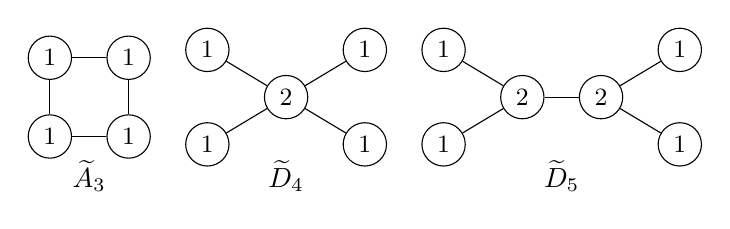
\begin{tikzpicture}[v/.style={circle,draw,minimum size=5.5mm,inner sep=0pt,font=\small}]
 \node[v] (a) at (0,0) {1}; \node[v] (b) at (1,0) {1};
 \node[v] (c) at (1,1) {1}; \node[v] (d) at (0,1) {1};
 \draw (a)--(b)--(c)--(d)--(a);
 \node at (.5,-.5) {$\widetilde A_3$};
 \node[v] (e) at (3,0.5) {2};
 \foreach \n/\x/\y in {f/2/1.1,g/2/-.1,h/4/1.1,i/4/-.1}
  {\node[v] (\n) at (\x,\y) {1}; \draw (e)--(\n);}
 \node at (3,-.5) {$\widetilde D_4$};
 \node[v] (j) at (6,0.5) {2}; \node[v] (k) at (7,0.5) {2};
 \draw (j)--(k);
 \foreach \n/\x/\y/\p in {l/5/1.1/j,m/5/-.1/j,n/8/1.1/k,o/8/-.1/k}
  {\node[v] (\n) at (\x,\y) {1}; \draw (\p)--(\n);}
 \node at (6.5,-.5) {$\widetilde D_5$};
\end{tikzpicture}

\small Diagramy cykliczny i dwucykliczne; w większym typie $D$
wydłuża się ścieżka wierzchołków wymiaru dwa.
\end{center}

\begin{center}
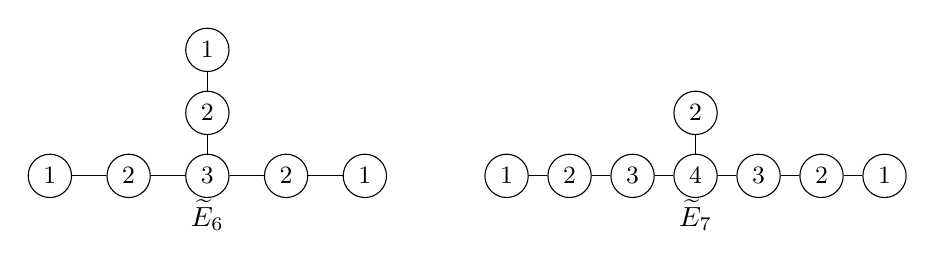
\begin{tikzpicture}[v/.style={circle,draw,minimum size=5.5mm,inner sep=0pt,font=\small}]
 \node[v] (c) at (2,0) {3};
 \node[v] (l1) at (1,0) {2}; \node[v] (l2) at (0,0) {1};
 \node[v] (r1) at (3,0) {2}; \node[v] (r2) at (4,0) {1};
 \node[v] (u1) at (2,.8) {2}; \node[v] (u2) at (2,1.6) {1};
 \draw (l2)--(l1)--(c)--(r1)--(r2); \draw (c)--(u1)--(u2);
 \node at (2,-.5) {$\widetilde E_6$};
 \node[v] (d) at (8.2,0) {4};
 \foreach \n/\x/\w in {a/5.8/1,b/6.6/2,e/7.4/3,f/9/3,g/9.8/2,h/10.6/1}
  {\node[v] (\n) at (\x,0) {\w};}
 \node[v] (u) at (8.2,.8) {2};
 \draw (a)--(b)--(e)--(d)--(f)--(g)--(h); \draw (d)--(u);
 \node at (8.2,-.5) {$\widetilde E_7$};
\end{tikzpicture}

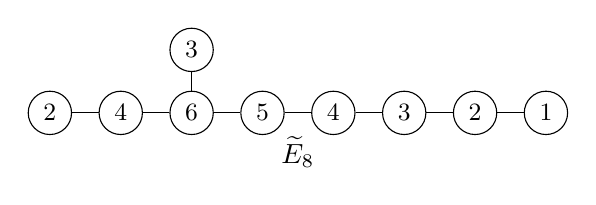
\begin{tikzpicture}[v/.style={circle,draw,minimum size=5.5mm,inner sep=0pt,font=\small}]
 \foreach \n/\x/\w in {a/0/2,b/.9/4,c/1.8/6,d/2.7/5,e/3.6/4,f/4.5/3,g/5.4/2,h/6.3/1}
  {\node[v] (\n) at (\x,0) {\w};}
 \node[v] (u) at (1.8,.8) {3};
 \draw (a)--(b)--(c)--(d)--(e)--(f)--(g)--(h); \draw (c)--(u);
 \node at (3.15,-.5) {$\widetilde E_8$};
\end{tikzpicture}

\small Diagramy wyjątkowe z wymiarami reprezentacji.
\end{center}

\begin{przyklad}[Odczytywanie iloczynów tensorowych]
Niech $G=2I$. Oznaczmy reprezentacje wzdłuż najdłuższego
ramienia od liścia przez $L_1,L_2,L_3,L_4,L_5,L_6$,
gdzie $\dim L_i=i$. Pozostałe reprezentacje oznaczmy
przez $M_3,M_4,M_2$, zgodnie z wymiarami i położeniem:
$M_3$ jest krótkim ramieniem, $M_4,M_2$ tworzą
ramię długości dwa. Mamy $L_1=\mathbb C$, $L_2=V$.
Z diagramu otrzymujemy
\[
\begin{aligned}
 V\otimes L_1&\simeq L_2,\\
 V\otimes L_i&\simeq L_{i-1}\oplus L_{i+1}\quad(2\le i\le5),\\
 V\otimes L_6&\simeq L_5\oplus M_3\oplus M_4,\\
 V\otimes M_3&\simeq L_6,\qquad
 V\otimes M_4\simeq L_6\oplus M_2,\qquad
 V\otimes M_2\simeq M_4.
\end{aligned}
\]
Przykładowo w trzecim wierszu $2\cdot6=5+3+4$.
Reprezentacje o tych samych wymiarach są rozróżnione
przez położenie w grafie, nie przez sam wymiar.
\end{przyklad}

\section{Potęgi symetryczne i pierścienie niezmienników}

\begin{twierdzenie}[Rekurencja McKaya]
\label{aa:tw:mckay-recurrence}
W oznaczeniach Definicji~\ref{aa:def:mckay} niech
$m_k$ będzie kolumną krotności reprezentacji $V_i$
w $\operatorname{Sym}^k V$, $k\ge0$.
Wówczas $m_0=e_0$, $m_1=Ae_0$ oraz
$m_{k+1}=Am_k-m_{k-1}$ dla $k\ge1$, gdzie $e_0$
jest wektorem jednostkowym przy reprezentacji trywialnej.
Szereg Hilberta pierścienia $\mathbb C[x,y]^G$ spełnia
\[
 H_G(z)=e_0^{\mathsf T}(I-zA+z^2 I)^{-1}e_0.
\]
Odwrotność rozumiemy w pierścieniu macierzy nad
$\mathbb C[[z]]$.
\end{twierdzenie}
\begin{proof}
Każdy $g\in G$ jest diagonalizowalny: jego wielomian
minimalny dzieli $X^{|G|}-1$, który nad $\mathbb C$
nie ma pierwiastków wielokrotnych. Wyznacznik
$g$ wynosi jeden, więc wartości własne to
$\lambda,\lambda^{-1}$. Charakter $\operatorname{Sym}^k V$ wynosi
$c_k(g)=\sum_{j=0}^k\lambda^{k-2j}$:
monomy stopnia $k$ w bazie wektorów własnych tworzą
bazę potęgi symetrycznej. Mnożenie przez
$\lambda+\lambda^{-1}$ daje wyrazy
$\lambda^{k+1},\lambda^{-k-1}$ po jednym razie,
a wszystkie pośrednie potęgi po dwa razy. Stąd
$\chi_V c_k=c_{k+1}+c_{k-1}$ dla $k\ge1$.
Z jednoznaczności rozkładu charakterów na bazę
charakterów nieprzywiedlnych
(Twierdzenie~\ref{aa:tw:characters-basis}) i symetrii $A$
wynika rekurencja: krotność $V_j$ w iloczynie
$V\otimes\operatorname{Sym}^k V$ jest równa
$\sum_i a_{ij}(m_k)_i=(Am_k)_j$, a po drugiej
stronie to $(m_{k+1})_j+(m_{k-1})_j$.
Dwa warunki początkowe wynikają
z $\operatorname{Sym}^0 V=\mathbb C$ i
$\operatorname{Sym}^1 V=V$.

Dla formalnego szeregu kolumn $M(z)=\sum_{k\ge0}m_kz^k$
mnożenie przez $I-zA+z^2I$ daje $e_0$, gdyż
współczynnik stały to $m_0$, liniowy to $m_1-Am_0=0$,
a wyższe współczynniki znikają z rekurencji.
Macierz ma wyraz stały $I$, więc ma odwrotność
formalną (rozwijamy szereg geometryczny macierzy
$zA-z^2I$). Niezdegenerowana forma
$(u,v)\mapsto\det(u,v)$ jest zachowywana przez $G$,
zatem $V\to V^*$, $u\mapsto\det(u,\cdot)$ jest
izomorfizmem reprezentacji. Jednorodna część
$\mathbb C[x,y]$ stopnia $k$ jest $\operatorname{Sym}^k V^*$,
a więc jest izomorficzna z $\operatorname{Sym}^k V$.
Wymiar jej przestrzeni wektorów ustalonych przez $G$
jest krotnością reprezentacji trywialnej (pozostałe
nieprzywiedlne reprezentacje nie mają wektorów ustalonych).
Stąd $H_G=e_0^{\mathsf T}M(z)$.
\end{proof}

\begin{przyklad}[Pierwsze niezmienniki dwudziestościenne]
W grafie $\widetilde E_8$ oznaczmy wektor jednostkowy
odpowiadający $L_i$ przez $e_{L_i}$, analogicznie
dla $M_j$. Z poprzedniej rekurencji
$m_0=e_{L_1}$, $m_1=e_{L_2}$, a dla $2\le k\le5$
otrzymujemy $m_k=e_{L_{k+1}}$ (odejmujemy jednego
sąsiada z poprzedniego kroku).
Następnie $m_6=e_{M_3}+e_{M_4}$, ponieważ
$Ae_{L_6}=e_{L_5}+e_{M_3}+e_{M_4}$.
Dla przykładu następne dwa kroki to
$m_7=A(e_{M_3}+e_{M_4})-e_{L_6}
=e_{L_6}+e_{M_2}$ oraz
$m_8=A(e_{L_6}+e_{M_2})-(e_{M_3}+e_{M_4})
=e_{L_5}+e_{M_4}$.
Powtarzając te działania otrzymujemy
\[
\begin{aligned}
 m_7&=e_{L_6}+e_{M_2},&
 m_8&=e_{L_5}+e_{M_4},\\
 m_9&=e_{L_4}+e_{L_6},&
 m_{10}&=e_{L_3}+e_{L_5}+e_{M_3},\\
 m_{11}&=e_{L_2}+e_{L_4}+e_{L_6},&
 m_{12}&=e_{L_1}+e_{L_3}+e_{L_5}+e_{M_4}.
\end{aligned}
\]
W szczególności pierwsze wystąpienie reprezentacji
trywialnej po stopniu zero następuje w stopniu $12$,
zgodnie z Twierdzeniem~\ref{aa:tw:exceptional-hilbert}.
\end{przyklad}

Otrzymana odpowiedniość dotyczy grafów reprezentacji
i typów równań pierścieni niezmienników z rozdziałów 53--54.
Geometryczna odpowiedniość między reprezentacjami
a krzywymi wyjątkowymi rezolucji minimalnej wymaga
osobnego dowodu; nie wyprowadzamy jej z samej
zgodności nazw diagramów.
